\chapter{Turbo Codes}
\label{ch:turbo-codes}

\begin{nontechnical}
\textbf{Turbo codes are like having two spell-checkers that help each other}---when one is unsure, the other provides hints, and they iterate back and forth until they agree. Revolutionary in 1993!

\textbf{The breakthrough:}
\begin{itemize}
\item \textbf{Before 1993:} Best codes were $\sim$3~dB from theoretical limit
\item \textbf{Turbo codes (1993):} Got within 0.5~dB of Shannon limit!
\item \textbf{Impact:} ``Impossible'' performance, shocked the world
\item \textbf{Today:} In 3G/4G phones, deep space, satellites
\end{itemize}

\textbf{How they work---Two encoders help each other:}

\textbf{Step 1: Encode data with TWO different convolutional encoders}
\begin{itemize}
\item Encoder 1: Sees data in original order
\item Encoder 2: Sees data scrambled (interleaved)
\item Send both encoded versions
\end{itemize}

\textbf{Step 2: Receiver iteratively decodes}
\begin{itemize}
\item Decoder 1: ``I think bit 5 is probably a 1... 80\% sure''
\item Decoder 2: ``I think bit 5 is definitely a 1... 95\% sure!''
\item Decoder 1: ``Oh! With that info, I'm now 98\% sure!''
\item They ping-pong back and forth $\sim$5--10 iterations
\item Final result: Near-perfect decoding!
\end{itemize}

\textbf{The magic---``Turbo'' analogy:}
\begin{itemize}
\item Like a turbo charger: Output feeds back to improve input
\item Each decoder's output improves the other's input
\item After several iterations, converges to correct answer
\item Hence: ``Turbo'' codes!
\end{itemize}

\textbf{Real-world use:}
\begin{itemize}
\item \textbf{3G (UMTS):} Turbo codes for data channels
\item \textbf{4G (LTE):} Turbo codes (before LDPC in 5G)
\item \textbf{Deep space:} Mars rovers use turbo codes
\item \textbf{Satellite phones:} Iridium, Globalstar
\item \textbf{Military:} Tactical communications
\end{itemize}

\textbf{Why ``revolutionary'' in 1993:}
\begin{itemize}
\item Shannon's limit (1948): Theoretical best = 0~dB $E_b/N_0$
\item Best codes before 1993: $\sim$3~dB from limit
\item Turbo codes: 0.5--1~dB from limit!
\item Engineers thought this was impossible!
\end{itemize}

\textbf{The famous 1993 paper:}
\begin{itemize}
\item Presented at ICC '93 conference
\item Audience: Stunned silence, then standing ovation
\item ``We must have made a mistake''---initial reaction
\item Verified by others: IT'S REAL!
\item Changed communication systems forever
\end{itemize}

\textbf{The iterative decoding process:}
\begin{center}
\begin{tabular}{@{}ll@{}}
\toprule
Iteration & Confidence Level \\
\midrule
1 & 60\% \\
2 & 80\% \\
3 & 95\% \\
4 & 99\% \\
5 & 99.9\% --- DONE! \\
\bottomrule
\end{tabular}
\end{center}

\textbf{Fun fact:} The inventors (Berrou, Glavieux, Thitimajshima) almost didn't publish because they thought they'd made a mistake---the performance seemed too good to be true. When they finally presented in 1993, it sparked a revolution in error correction!
\end{nontechnical}

\section{Overview}

\textbf{Turbo codes} achieve \textbf{near-Shannon-limit} performance (within 0.5--1~dB of capacity), representing one of the most significant breakthroughs in coding theory since Shannon's original work in 1948.

\begin{keyconcept}
Turbo codes provide \textbf{unprecedented error correction performance} through parallel concatenation of two recursive systematic convolutional (RSC) encoders separated by an interleaver, combined with iterative soft-output decoding. This architecture achieves BER of $10^{-5}$ at $E_b/N_0 \approx 0.7$~dB for rate 1/2 BPSK---only 0.5~dB from the Shannon limit.
\end{keyconcept}

\textbf{Key innovation:} The breakthrough lies in the iterative exchange of \textbf{extrinsic information} between two soft-input soft-output (SISO) decoders. Each decoder refines its estimates using information from the other, creating a feedback loop that converges toward the correct codeword.

\textbf{Discovery:} Claude Berrou, Alain Glavieux, and Punya Thitimajshima presented turbo codes at the 1993 IEEE International Communication Conference (ICC), stunning the communications community with performance previously thought impossible.

\textbf{Applications:}
\begin{itemize}
\item 3G cellular (UMTS/WCDMA): Data channels up to 2~Mbps
\item 4G LTE: All data channels (until 5G transition to LDPC)
\item Deep space: Mars rovers, Voyager missions, New Horizons
\item Satellite communications: DVB-RCS, Inmarsat, Iridium
\item Military communications: Tactical data links
\end{itemize}

\section{Mathematical Description}

\subsection{Code Structure}

A rate $R_c = 1/3$ turbo code encodes an input data block $\mathbf{d} = [d_1, d_2, \ldots, d_K]$ into a codeword $\mathbf{c}$ of length $3K$ bits.

\textbf{Encoding function:}
\begin{equation}
\mathbf{c} = [\mathbf{d}, \mathbf{p}_1, \mathbf{p}_2] = \text{Encode}(\mathbf{d}, \pi, G_1, G_2)
\end{equation}

where:
\begin{itemize}
\item $\mathbf{d}$ = systematic bits (original data)
\item $\mathbf{p}_1$ = parity bits from encoder 1
\item $\mathbf{p}_2$ = parity bits from encoder 2
\item $\pi$ = interleaver permutation
\item $G_1, G_2$ = generator polynomials for RSC encoders
\end{itemize}

\subsection{Generator Polynomial Representation}

An RSC encoder with constraint length $K$ is described by two polynomials:

\begin{equation}
G(D) = \left[1, \frac{g(D)}{h(D)}\right]
\end{equation}

where:
\begin{itemize}
\item $h(D)$ = feedback polynomial (determines recursion)
\item $g(D)$ = feedforward polynomial (generates parity)
\item $D$ = delay operator
\end{itemize}

\textbf{Example: LTE turbo code ($K=4$)}
\begin{equation}
\begin{aligned}
h(D) &= 1 + D^2 + D^3 \quad \text{(feedback: } 15_8\text{)} \\
g(D) &= 1 + D + D^3 \quad \text{(feedforward: } 13_8\text{)}
\end{aligned}
\end{equation}

\subsection{Iterative Decoding Equations}

The turbo decoder computes log-likelihood ratios (LLRs) through iterative refinement:

\begin{equation}
L^{(i)}(d_k) = L_c(d_k) + L_a^{(i)}(d_k) + L_e^{(i)}(d_k)
\end{equation}

\textbf{Extrinsic information update:}
\begin{equation}
L_e^{(i)}(d_k) = \text{BCJR}(L_c, L_a^{(i)}) - L_c(d_k) - L_a^{(i)}(d_k)
\end{equation}

\textbf{A priori information for next iteration:}
\begin{equation}
L_a^{(i+1)}(\mathbf{d}) = \pi^{-1}\left(L_e^{(i)}(\mathbf{d}')\right)
\end{equation}

\textbf{Convergence criterion:}
\begin{equation}
\max_{k} \left| L^{(i)}(d_k) - L^{(i-1)}(d_k) \right| < \epsilon \quad \text{or} \quad i = N_{\max}
\end{equation}

\section{Turbo Encoder Architecture}

\subsection{Parallel Concatenated Convolutional Codes (PCCC)}

Turbo codes employ a \textbf{parallel concatenated} structure consisting of two recursive systematic convolutional (RSC) encoders separated by an interleaver:

\begin{center}
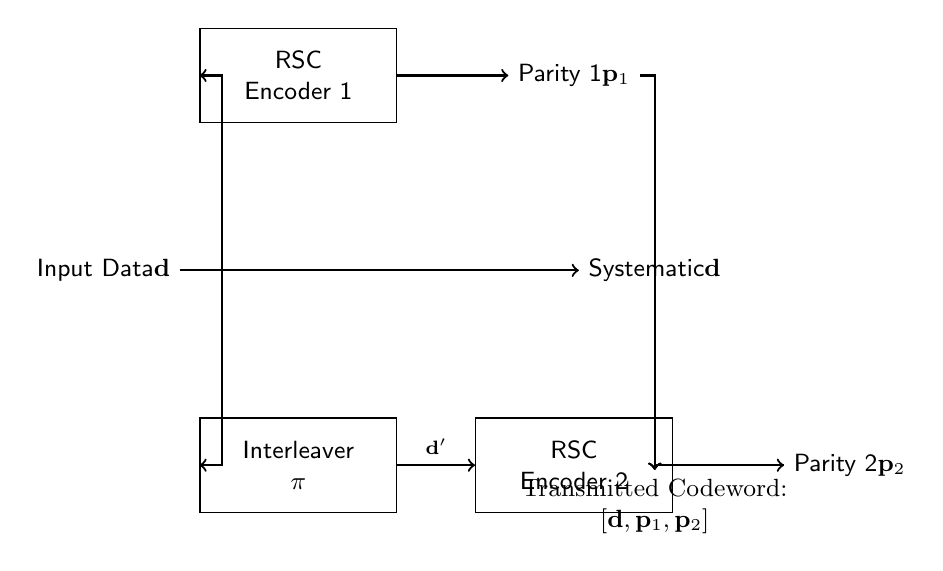
\begin{tikzpicture}[
  block/.style={rectangle, draw, minimum width=2.5cm, minimum height=1.2cm, font=\sffamily\small, align=center},
  node distance=2.5cm,
  font=\small
]
% Input
\node (input) {\sffamily Input Data\\$\mathbf{d}$};

% Upper path - RSC Encoder 1
\node[block, above right of=input, node distance=3.5cm] (rsc1) {RSC\\Encoder 1};
\node[right of=rsc1, node distance=3.5cm] (p1) {\sffamily Parity 1\\$\mathbf{p}_1$};

% Middle path - Systematic
\node[right of=input, node distance=7cm] (sys) {\sffamily Systematic\\$\mathbf{d}$};

% Lower path - Interleaver and RSC Encoder 2
\node[block, below right of=input, node distance=3.5cm] (int) {Interleaver\\$\pi$};
\node[block, right of=int, node distance=3.5cm] (rsc2) {RSC\\Encoder 2};
\node[right of=rsc2, node distance=3.5cm] (p2) {\sffamily Parity 2\\$\mathbf{p}_2$};

% Arrows
\draw[->,thick] (input) -- ++(1.5,0) |- (rsc1);
\draw[->,thick] (input) -- (sys);
\draw[->,thick] (input) -- ++(1.5,0) |- (int);
\draw[->,thick] (rsc1) -- (p1);
\draw[->,thick] (int) -- node[above,font=\scriptsize] {$\mathbf{d}'$} (rsc2);
\draw[->,thick] (rsc2) -- (p2);

% Output block
\node[below of=sys, node distance=3cm, align=center, font=\small] (output) {Transmitted Codeword:\\$[\mathbf{d}, \mathbf{p}_1, \mathbf{p}_2]$};
\draw[->,thick] (sys) -- (output);
\draw[->,thick] (p1) -| (output);
\draw[->,thick] (p2) -| (output);
\end{tikzpicture}
\end{center}

\textbf{Components:}
\begin{enumerate}
\item \textbf{Two RSC encoders:} Recursive Systematic Convolutional encoders with identical or complementary generator polynomials
\item \textbf{Interleaver $\pi$:} Pseudo-random permutation that scrambles the input bit sequence
\item \textbf{Systematic output:} Original data transmitted uncoded (ensures minimum rate 1/3)
\end{enumerate}

\textbf{Output codeword:} For each $K$-bit input block, the encoder produces:
\begin{itemize}
\item $K$ systematic bits (original data)
\item $K$ parity bits from encoder 1
\item $K$ parity bits from encoder 2
\item \textbf{Code rate:} $R = K/(3K) = 1/3$ (can be increased via puncturing)
\end{itemize}

\subsection{Recursive Systematic Convolutional (RSC) Encoder}

The RSC encoder is fundamental to turbo code performance. Unlike standard convolutional codes, RSC encoders feature \textbf{feedback}, which creates an infinite impulse response (IIR) structure essential for effective iterative decoding.

\begin{center}
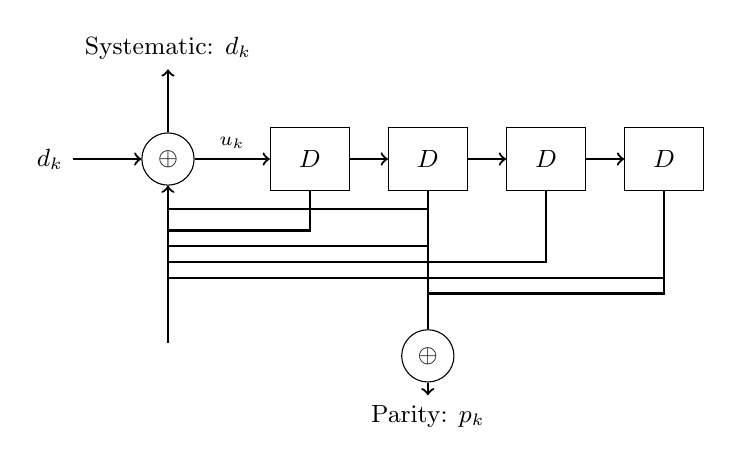
\begin{tikzpicture}[
  block/.style={rectangle, draw, minimum width=1cm, minimum height=0.8cm, font=\sffamily\small},
  node distance=1.5cm,
  font=\small
]
% Input
\node (input) {$d_k$};

% Feedback summing junction
\node[circle, draw, right of=input, node distance=1.5cm] (sum1) {$\oplus$};

% Shift register stages
\node[block, right of=sum1, node distance=1.8cm] (s1) {$D$};
\node[block, right of=s1, node distance=1.5cm] (s2) {$D$};
\node[block, right of=s2, node distance=1.5cm] (s3) {$D$};
\node[block, right of=s3, node distance=1.5cm] (s4) {$D$};

% Feedback path
\draw[->,thick] (input) -- (sum1);
\draw[->,thick] (sum1) -- node[above,font=\scriptsize] {$u_k$} (s1);
\draw[->,thick] (s1) -- (s2);
\draw[->,thick] (s2) -- (s3);
\draw[->,thick] (s3) -- (s4);

% Feedback taps (for 37 octal = 011111)
\draw[thick] (s1.south) -- ++(0,-0.5) -| ([yshift=-2cm]sum1.south);
\draw[thick] (s2.south) -- ++(0,-0.7) -| ([yshift=-2cm]sum1.south);
\draw[thick] (s3.south) -- ++(0,-0.9) -| ([yshift=-2cm]sum1.south);
\draw[thick] (s4.south) -- ++(0,-1.1) -| ([yshift=-2cm]sum1.south);
\draw[->,thick] ([yshift=-2cm]sum1.south) -- (sum1);

% Systematic output
\draw[->,thick] (sum1.north) -- ++(0,0.8) node[above] {Systematic: $d_k$};

% Parity output summing junction
\node[circle, draw, below of=s2, node distance=2.5cm] (sum2) {$\oplus$};
\draw[thick] (sum1.south) -- ++(0,-0.3) -| (sum2);
\draw[thick] (s4.south) -- ++(0,-1.3) -| (sum2);
\draw[->,thick] (sum2) -- ++(0,-0.5) node[below] {Parity: $p_k$};

\end{tikzpicture}
\end{center}

\textbf{Key properties:}
\begin{itemize}
\item \textbf{Recursive:} Feedback path from register outputs to input creates IIR
\item \textbf{Systematic:} One output equals the input (provides uncoded reference)
\item \textbf{Memory:} Constraint length $K$ determines number of states ($2^{K-1}$)
\end{itemize}

\subsubsection{Standard RSC Generator Polynomials}

\textbf{Example: RSC (37, 21) Octal (LTE Standard)}

\textbf{Generator polynomials:}
\begin{equation}
\begin{aligned}
G_{\text{feedback}} &= 37_8 = 011111_2 \\
G_{\text{feedforward}} &= 21_8 = 010001_2
\end{aligned}
\end{equation}

\textbf{Parameters:}
\begin{itemize}
\item Constraint length: $K = 5$
\item Number of states: $2^{K-1} = 16$
\item Code rate: $R = 1/2$ (1 systematic + 1 parity per input bit)
\end{itemize}

\begin{warningbox}
\textbf{Why recursive?} Non-recursive encoders produce finite-weight outputs for low-weight inputs. RSC encoders spread input errors across many output bits through feedback, dramatically improving the distance properties of the concatenated code. This is \textbf{essential} for near-capacity performance.
\end{warningbox}

\subsection{Interleaver Design}

The interleaver is the \textbf{heart of the turbo code}. It breaks the correlation between the two encoder inputs, ensuring that low-weight sequences for one encoder become high-weight sequences for the other.

\subsubsection{Interleaver Operation}

An interleaver $\pi$ performs a pseudo-random permutation on the input data:
\begin{equation}
\mathbf{d}' = \pi(\mathbf{d}) = [d_{\pi(1)}, d_{\pi(2)}, \ldots, d_{\pi(K)}]
\end{equation}
where $\pi(i)$ maps input position $i$ to output position.

\begin{center}
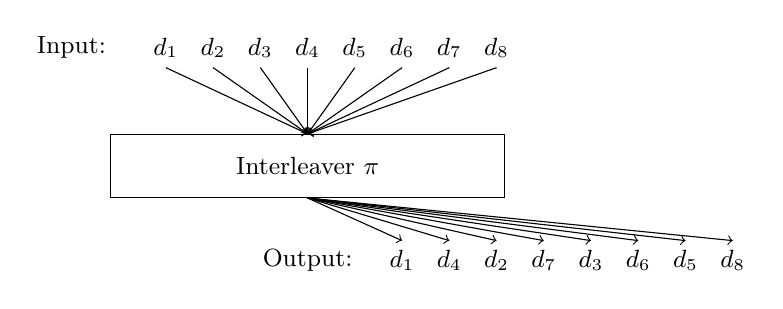
\begin{tikzpicture}[
  node distance=0.6cm,
  font=\small
]
% Input sequence
\node (in_label) {Input:};
\node[right of=in_label, node distance=1.2cm] (in1) {$d_1$};
\node[right of=in1] (in2) {$d_2$};
\node[right of=in2] (in3) {$d_3$};
\node[right of=in3] (in4) {$d_4$};
\node[right of=in4] (in5) {$d_5$};
\node[right of=in5] (in6) {$d_6$};
\node[right of=in6] (in7) {$d_7$};
\node[right of=in7] (in8) {$d_8$};

% Interleaver box
\node[below of=in4, node distance=1.5cm, draw, minimum width=5cm, minimum height=0.8cm] (int) {Interleaver $\pi$};

% Output sequence
\node[below of=int, node distance=1.2cm] (out_label) {Output:};
\node[right of=out_label, node distance=1.2cm] (out1) {$d_1$};
\node[right of=out1] (out2) {$d_4$};
\node[right of=out2] (out3) {$d_2$};
\node[right of=out3] (out4) {$d_7$};
\node[right of=out4] (out5) {$d_3$};
\node[right of=out5] (out6) {$d_6$};
\node[right of=out6] (out7) {$d_5$};
\node[right of=out7] (out8) {$d_8$};

% Arrows showing permutation
\draw[->,thin] (in1.south) -- (int.north);
\draw[->,thin] (in2.south) -- (int.north);
\draw[->,thin] (in3.south) -- (int.north);
\draw[->,thin] (in4.south) -- (int.north);
\draw[->,thin] (in5.south) -- (int.north);
\draw[->,thin] (in6.south) -- (int.north);
\draw[->,thin] (in7.south) -- (int.north);
\draw[->,thin] (in8.south) -- (int.north);

\draw[->,thin] (int.south) -- (out1.north);
\draw[->,thin] (int.south) -- (out2.north);
\draw[->,thin] (int.south) -- (out3.north);
\draw[->,thin] (int.south) -- (out4.north);
\draw[->,thin] (int.south) -- (out5.north);
\draw[->,thin] (int.south) -- (out6.north);
\draw[->,thin] (int.south) -- (out7.north);
\draw[->,thin] (int.south) -- (out8.north);
\end{tikzpicture}
\end{center}

\subsubsection{Interleaver Types}

\textbf{1. Random Interleaver}
\begin{itemize}
\item Completely pseudo-random permutation
\item Best performance for large block sizes
\item No structure; requires lookup table storage
\end{itemize}

\textbf{2. Block Interleaver}
\begin{itemize}
\item Write data row-wise, read column-wise (or vice versa)
\item Simple implementation (modular arithmetic)
\item Moderate performance; predictable structure
\end{itemize}

\textbf{3. S-Random Interleaver}
\begin{itemize}
\item Constrained randomness to avoid short-distance mappings
\item Better distance properties than pure random
\item Industry standard for many applications
\end{itemize}

\textbf{4. Quadratic Permutation Polynomial (QPP)}
\begin{itemize}
\item Used in LTE: $\pi(i) = (f_1 i + f_2 i^2) \mod K$
\item Contention-free parallel access
\item Optimized for hardware implementation
\end{itemize}

\subsubsection{Why Interleaving Works}

Consider a low-weight input sequence producing poor distance properties:

\begin{center}
\begin{tabular}{@{}lll@{}}
\toprule
Stage & Sequence & Weight \\
\midrule
Input & $[1, 1, 1, 1, 1, 0, 0, 0]$ & 5 \\
Encoder 1 parity & Low-weight output & Poor \\
\midrule
After interleaver & $[1, 0, 1, 0, 1, 0, 1, 0]$ & 5 \\
Encoder 2 parity & High-weight output & Good \\
\bottomrule
\end{tabular}
\end{center}

\textbf{Result:} Combined code has high minimum distance $\rightarrow$ excellent error correction.

\subsubsection{S-Random Interleaver Design}

\textbf{Constraint:} For any two indices $i$ and $j$:
\begin{equation}
|i - j| < S \quad \Rightarrow \quad |\pi(i) - \pi(j)| \geq S
\end{equation}

\textbf{Typical value:} $S = \sqrt{K}$ where $K$ is block length

\textbf{Benefit:} Prevents low-weight error patterns from being preserved through both encoders, eliminating weak codewords that create error floors.

\textbf{Block size:} Typically $K = 1{,}000$--$10{,}000$ bits
\begin{itemize}
\item Longer interleaver $\rightarrow$ better performance
\item Longer interleaver $\rightarrow$ higher latency and memory
\end{itemize}

\section{Encoding Process}

\subsection{Complete Encoding Steps}

\textbf{Input:} Data block $\mathbf{d} = [d_1, d_2, \ldots, d_K]$ of length $K$ bits

\textbf{Encoding algorithm:}

\begin{enumerate}
\item \textbf{Encoder 1:} Encode $\mathbf{d}$ through RSC encoder 1
  \begin{equation}
  \mathbf{p}_1 = \text{RSC}_1(\mathbf{d})
  \end{equation}

\item \textbf{Interleave:} Apply permutation $\pi$ to input data
  \begin{equation}
  \mathbf{d}' = \pi(\mathbf{d})
  \end{equation}

\item \textbf{Encoder 2:} Encode interleaved data through RSC encoder 2
  \begin{equation}
  \mathbf{p}_2 = \text{RSC}_2(\mathbf{d}')
  \end{equation}

\item \textbf{Transmit:} Send systematic bits and both parity sequences
  \begin{equation}
  \mathbf{c} = [\mathbf{d}, \mathbf{p}_1, \mathbf{p}_2]
  \end{equation}
  \textbf{Code rate:} $R = K/(K + K + K) = 1/3$
\end{enumerate}

\subsection{Rate Matching (Puncturing)}

Higher code rates are achieved by \textbf{puncturing} (deleting) selected parity bits according to a periodic pattern.

\textbf{Example: Rate 1/3 $\rightarrow$ Rate 1/2}

Apply alternating puncturing pattern to parity streams:

\begin{center}
\begin{tabular}{@{}ccccc@{}}
\toprule
Time & Systematic & Parity 1 & Parity 2 & Transmitted \\
\midrule
1 & $d_1$ & $p_{11}$ & \cancel{$p_{21}$} & $d_1, p_{11}$ \\
2 & $d_2$ & \cancel{$p_{12}$} & $p_{22}$ & $d_2, p_{22}$ \\
3 & $d_3$ & $p_{13}$ & \cancel{$p_{23}$} & $d_3, p_{13}$ \\
4 & $d_4$ & \cancel{$p_{14}$} & $p_{24}$ & $d_4, p_{24}$ \\
\bottomrule
\end{tabular}
\end{center}

\textbf{Result:} Transmit 4 systematic + 4 parity = 8 symbols for 4 information bits $\rightarrow$ Rate = $4/8 = 1/2$

\textbf{Common code rates:}
\begin{itemize}
\item Rate 1/3: No puncturing (parent code)
\item Rate 1/2: Alternating puncturing (50\% parity bits deleted)
\item Rate 2/3: Heavy puncturing (66\% parity bits deleted)
\item Rate 3/4: Very aggressive puncturing (75\% parity bits deleted)
\end{itemize}

\begin{calloutbox}{Trade-off: Code Rate vs. Performance}
Higher code rates increase spectral efficiency but reduce error correction capability. The optimal rate depends on channel conditions:
\begin{itemize}
\item \textbf{Good channel (high SNR):} Use rate 2/3 or 3/4
\item \textbf{Poor channel (low SNR):} Use rate 1/3 or 1/2
\item \textbf{Adaptive systems:} Switch rates based on measured SNR (e.g., LTE AMC)
\end{itemize}
\end{calloutbox}

\section{Iterative Decoding}

The \textbf{iterative decoding algorithm} is the key innovation that enables near-Shannon-limit performance. Two soft-input soft-output (SISO) decoders exchange \textbf{extrinsic information}, refining their estimates through multiple iterations.

\subsection{Turbo Decoder Architecture}

\begin{center}
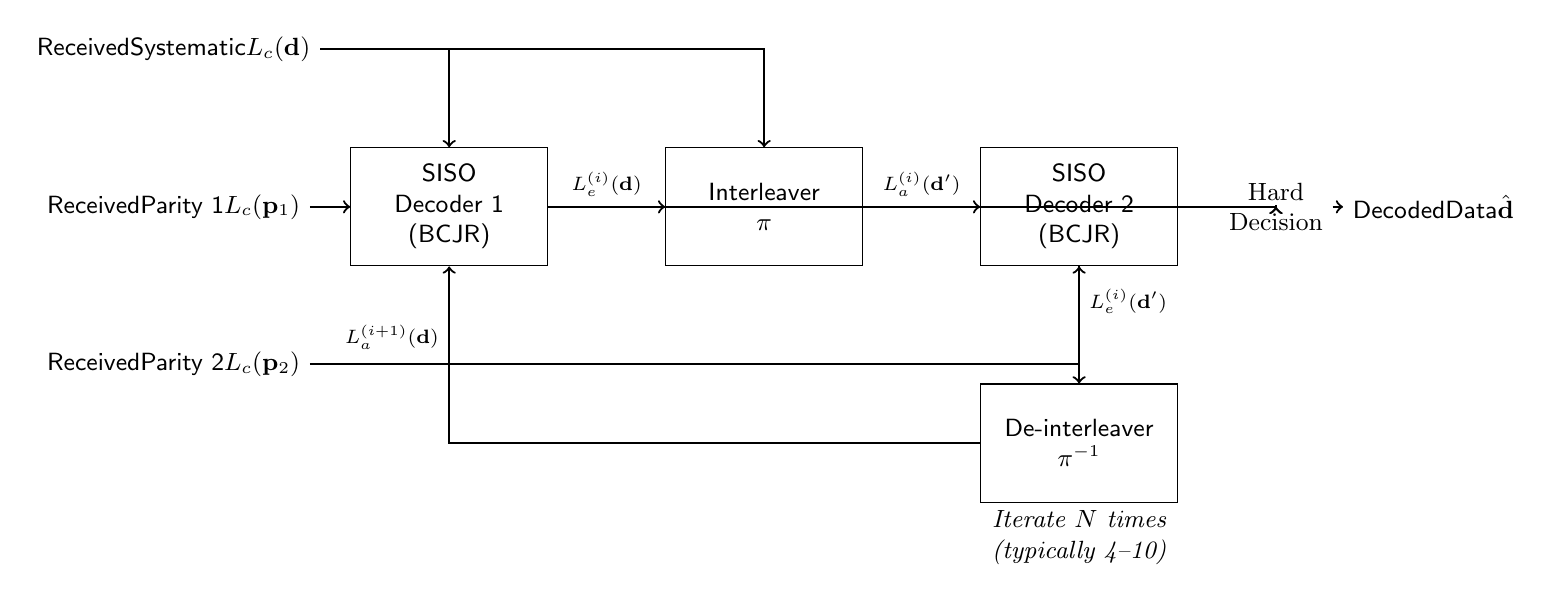
\begin{tikzpicture}[
  block/.style={rectangle, draw, minimum width=2.5cm, minimum height=1.5cm, font=\sffamily\small, align=center},
  node distance=3cm,
  font=\small
]
% Received signals
\node (rx_sys) at (0,2) {\sffamily Received\\Systematic\\$L_c(\mathbf{d})$};
\node (rx_p1) at (0,0) {\sffamily Received\\Parity 1\\$L_c(\mathbf{p}_1)$};
\node (rx_p2) at (0,-2) {\sffamily Received\\Parity 2\\$L_c(\mathbf{p}_2)$};

% Decoder 1
\node[block, right of=rx_p1, node distance=3.5cm] (dec1) {SISO\\Decoder 1\\(BCJR)};

% Interleaver
\node[block, right of=dec1, node distance=4cm] (int) {Interleaver\\$\pi$};

% Decoder 2
\node[block, right of=int, node distance=4cm] (dec2) {SISO\\Decoder 2\\(BCJR)};

% De-interleaver
\node[block, below of=dec2, node distance=3cm] (deint) {De-interleaver\\$\pi^{-1}$};

% Decision
\node[right of=dec1, node distance=10.5cm, align=center] (decision) {Hard\\Decision};

% Arrows
\draw[->,thick] (rx_sys) -| (dec1);
\draw[->,thick] (rx_p1) -- (dec1);

\draw[->,thick] (dec1) -- node[above,font=\scriptsize] {$L_e^{(i)}(\mathbf{d})$} (int);
\draw[->,thick] (int) -- node[above,font=\scriptsize] {$L_a^{(i)}(\mathbf{d}')$} (dec2);

\draw[->,thick] (rx_sys) -| (int);
\draw[->,thick] (rx_p2) -| (dec2);

\draw[->,thick] (dec2) -- node[right,font=\scriptsize,pos=0.3] {$L_e^{(i)}(\mathbf{d}')$} (deint);
\draw[->,thick] (deint) -| node[left,font=\scriptsize,pos=0.8] {$L_a^{(i+1)}(\mathbf{d})$} (dec1);

\draw[->,thick] (dec1.east) -| (decision);
\draw[->,thick] (dec2.east) -| (decision);

\node[right of=decision, node distance=2cm] (output) {\sffamily Decoded\\Data\\$\hat{\mathbf{d}}$};
\draw[->,thick] (decision) -- (output);

% Iteration label
\node[below of=deint, node distance=1.2cm, align=center, font=\small\itshape] {Iterate $N$ times\\(typically 4--10)};

\end{tikzpicture}
\end{center}

\textbf{Components:}
\begin{itemize}
\item \textbf{SISO Decoder:} Soft-Input Soft-Output decoder using BCJR or SOVA algorithm
\item \textbf{Extrinsic information $L_e$:} New information computed by decoder, excluding a priori knowledge
\item \textbf{A priori information $L_a$:} Information from the other decoder
\item \textbf{Iteration:} Decoders alternate, passing improved soft estimates
\end{itemize}

\subsection{Log-Likelihood Ratios (LLRs)}

Turbo decoding operates on \textbf{soft information} represented as log-likelihood ratios (LLRs).

\textbf{LLR definition for bit $d_k$:}
\begin{equation}
L(d_k) = \log\frac{P(d_k = 0 \mid \text{received})}{P(d_k = 1 \mid \text{received})}
\label{eq:llr-definition}
\end{equation}

\textbf{Interpretation:}
\begin{itemize}
\item $L(d_k) > 0$ $\rightarrow$ bit $d_k$ is likely 0
\item $L(d_k) < 0$ $\rightarrow$ bit $d_k$ is likely 1
\item $|L(d_k)|$ $\rightarrow$ confidence (magnitude = reliability)
\end{itemize}

\textbf{LLR decomposition:}
\begin{equation}
L(d_k) = L_c(d_k) + L_a(d_k) + L_e(d_k)
\label{eq:llr-decomposition}
\end{equation}

where:
\begin{itemize}
\item $L_c(d_k)$ = \textbf{Channel LLR} (from demodulator, based on received signal)
\item $L_a(d_k)$ = \textbf{A priori LLR} (from other decoder in previous iteration)
\item $L_e(d_k)$ = \textbf{Extrinsic LLR} (new information computed by this decoder)
\end{itemize}

\textbf{Channel LLR for BPSK in AWGN:}
\begin{equation}
L_c(d_k) = \frac{4 E_s}{N_0} \cdot r_k
\label{eq:channel-llr}
\end{equation}
where $r_k$ is the received sample and $E_s/N_0$ is the symbol SNR.

\subsection{Iterative Decoding Algorithm}

\textbf{Iteration $i$ (for $i = 1, 2, \ldots, N$):}

\begin{enumerate}
\item \textbf{Decoder 1 (SISO):}
  \begin{itemize}
  \item \textbf{Input:} $L_c(\mathbf{d})$, $L_c(\mathbf{p}_1)$, $L_a^{(i)}(\mathbf{d})$ (from Decoder 2)
  \item \textbf{Compute:} Run BCJR algorithm on trellis
  \item \textbf{Output:} Extrinsic information $L_e^{(i)}(\mathbf{d})$
  \begin{equation}
  L_e^{(i)}(d_k) = L_1^{(i)}(d_k) - L_c(d_k) - L_a^{(i)}(d_k)
  \end{equation}
  \end{itemize}

\item \textbf{Interleave extrinsic information:}
  \begin{equation}
  L_e^{(i)}(\mathbf{d}') = \pi(L_e^{(i)}(\mathbf{d}))
  \end{equation}

\item \textbf{Decoder 2 (SISO):}
  \begin{itemize}
  \item \textbf{Input:} $L_c(\mathbf{d}')$, $L_c(\mathbf{p}_2)$, $L_a^{(i)}(\mathbf{d}') = L_e^{(i)}(\mathbf{d}')$
  \item \textbf{Compute:} Run BCJR algorithm on interleaved trellis
  \item \textbf{Output:} Extrinsic information $L_e^{(i)}(\mathbf{d}')$
  \begin{equation}
  L_e^{(i)}(d_k') = L_2^{(i)}(d_k') - L_c(d_k') - L_a^{(i)}(d_k')
  \end{equation}
  \end{itemize}

\item \textbf{De-interleave for next iteration:}
  \begin{equation}
  L_a^{(i+1)}(\mathbf{d}) = \pi^{-1}(L_e^{(i)}(\mathbf{d}'))
  \end{equation}

\item \textbf{Repeat} for $N$ iterations (typically 4--10)

\item \textbf{Hard decision after final iteration:}
  \begin{equation}
  \hat{d}_k = \begin{cases}
  0 & \text{if } L_1^{(N)}(d_k) + L_2^{(N)}(d_k) > 0 \\
  1 & \text{if } L_1^{(N)}(d_k) + L_2^{(N)}(d_k) < 0
  \end{cases}
  \label{eq:hard-decision}
  \end{equation}
\end{enumerate}

\begin{keyconcept}
\textbf{Why iterative decoding works:} Each decoder provides \textbf{extrinsic information}---new knowledge derived from its parity checks that the other decoder doesn't have. By exchanging extrinsic information iteratively:
\begin{itemize}
\item Decoder 1 uses channel + parity 1 $\rightarrow$ produces soft estimates
\item Decoder 2 uses channel + parity 2 + \textbf{extrinsic from Dec1} $\rightarrow$ refines estimates
\item Decoder 1 uses \textbf{extrinsic from Dec2} $\rightarrow$ further refinement
\item LLRs converge to high magnitude (high confidence) after $\sim$4--10 iterations
\end{itemize}

\textbf{Analogy:} Two experts analyzing a problem from different perspectives, iteratively sharing insights until reaching consensus.
\end{keyconcept}

\section{BCJR Algorithm (MAP Decoding)}

The \textbf{Bahl-Cocke-Jelinek-Raviv (BCJR)} algorithm is the optimal soft-output decoder for convolutional codes. It computes the \textbf{maximum a posteriori (MAP)} probability for each bit given all received data.

\subsection{Forward-Backward Algorithm}

The BCJR algorithm operates in two passes through the trellis:

\subsubsection{Forward Recursion (Alpha)}

Compute forward state metrics $\alpha_k(s)$ representing probability of being in state $s$ at time $k$:
\begin{equation}
\alpha_k(s) = \sum_{s' \in \mathcal{S}} \alpha_{k-1}(s') \cdot \gamma_k(s', s)
\label{eq:alpha-recursion}
\end{equation}

\textbf{Initialization:} $\alpha_0(s_0) = 1$, $\alpha_0(s) = 0$ for $s \neq s_0$

\subsubsection{Backward Recursion (Beta)}

Compute backward state metrics $\beta_k(s)$ representing probability of future observations given state $s$ at time $k$:
\begin{equation}
\beta_{k-1}(s') = \sum_{s \in \mathcal{S}} \beta_k(s) \cdot \gamma_k(s', s)
\label{eq:beta-recursion}
\end{equation}

\textbf{Initialization:} $\beta_K(s_K) = 1$, $\beta_K(s) = 0$ for $s \neq s_K$ (assuming known final state)

\subsubsection{Branch Metric (Gamma)}

Branch metric represents probability of transition $s' \rightarrow s$ given received symbols:
\begin{equation}
\gamma_k(s', s) = P(r_k \mid s' \rightarrow s) \cdot P(s' \rightarrow s)
\label{eq:gamma-metric}
\end{equation}

For AWGN channel with BPSK:
\begin{equation}
\gamma_k(s', s) = \exp\left(\frac{2 E_s}{N_0} r_k \cdot c_k(s', s)\right) \cdot P_a(d_k)
\end{equation}
where $c_k(s', s)$ is the transmitted symbol for transition $s' \rightarrow s$ and $P_a(d_k)$ is the a priori probability.

\subsection{LLR Computation}

The output LLR for bit $d_k$ is computed from forward/backward metrics:
\begin{equation}
L(d_k) = \log\frac{\sum_{(s',s): d_k=0} \alpha_{k-1}(s') \cdot \gamma_k(s',s) \cdot \beta_k(s)}{\sum_{(s',s): d_k=1} \alpha_{k-1}(s') \cdot \gamma_k(s',s) \cdot \beta_k(s)}
\label{eq:bcjr-llr}
\end{equation}

\textbf{Complexity:}
\begin{itemize}
\item Number of states: $|\mathcal{S}| = 2^{K-1}$ where $K$ is constraint length
\item Operations per bit: $O(|\mathcal{S}|^2) = O(2^{2(K-1)})$
\item For $K = 5$: $2^8 = 256$ operations per bit (manageable)
\item For $K = 7$: $2^{12} = 4096$ operations per bit (higher complexity)
\end{itemize}

\begin{center}
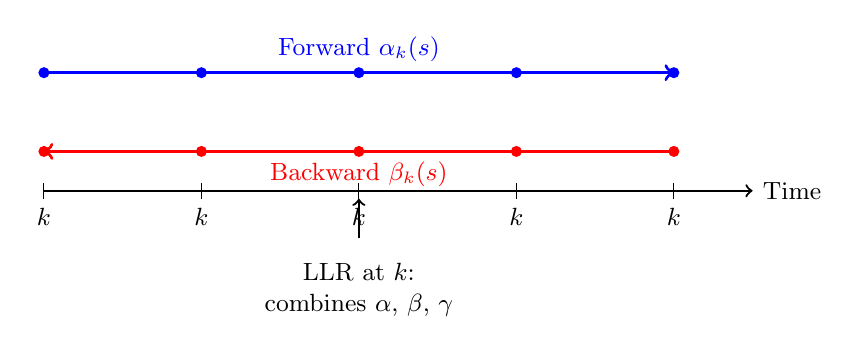
\begin{tikzpicture}[
  node distance=2cm,
  font=\small
]
% Timeline
\draw[->,thick] (0,0) -- (9,0) node[right] {Time};
\foreach \x in {0,2,4,6,8} {
  \draw (\x,0.1) -- (\x,-0.1) node[below] {$k$};
}

% Alpha forward
\draw[->,very thick,blue] (0,1.5) -- (8,1.5) node[midway,above] {Forward $\alpha_k(s)$};
\foreach \x in {0,2,4,6,8} {
  \fill[blue] (\x,1.5) circle (2pt);
}

% Beta backward
\draw[<-,very thick,red] (0,0.5) -- (8,0.5) node[midway,below] {Backward $\beta_k(s)$};
\foreach \x in {0,2,4,6,8} {
  \fill[red] (\x,0.5) circle (2pt);
}

% LLR computation point
\node[below,align=center] at (4,-0.8) {LLR at $k$:\\combines $\alpha$, $\beta$, $\gamma$};
\draw[->,thick] (4,-0.6) -- (4,-0.1);

\end{tikzpicture}
\end{center}

\subsection{Log-Domain BCJR}

To avoid numerical underflow, BCJR is typically implemented in the log domain:
\begin{equation}
\tilde{\alpha}_k(s) = \log(\alpha_k(s)), \quad \tilde{\beta}_k(s) = \log(\beta_k(s))
\end{equation}

Using the Jacobian logarithm:
\begin{equation}
\log(e^a + e^b) = \max(a, b) + \log(1 + e^{-|a-b|})
\label{eq:jacobian-log}
\end{equation}

\textbf{Max-Log-MAP approximation:} Drop the correction term for reduced complexity:
\begin{equation}
\log(e^a + e^b) \approx \max(a, b)
\end{equation}
\textbf{Performance loss:} Approximately 0.3--0.5~dB compared to exact log-MAP

\section{Performance Analysis}

\subsection{Bit Error Rate Performance}

Turbo codes achieve remarkable BER performance, approaching the Shannon limit.

\textbf{Typical performance} (Rate 1/2, $K=4$, random interleaver, 10 iterations, BPSK modulation):

\begin{center}
\begin{tabular}{@{}cccc@{}}
\toprule
$E_b/N_0$ (dB) & Uncoded BPSK & Turbo Code & Notes \\
\midrule
$-1.6$ & $2.7 \times 10^{-1}$ & --- & Shannon limit (capacity) \\
$0.0$ & $7.9 \times 10^{-2}$ & $1.0 \times 10^{-2}$ & \\
$0.5$ & $4.0 \times 10^{-2}$ & $1.0 \times 10^{-3}$ & \\
$0.7$ & $3.0 \times 10^{-2}$ & $1.0 \times 10^{-5}$ & Gap = 0.5~dB \\
$1.0$ & $2.0 \times 10^{-2}$ & $1.0 \times 10^{-6}$ & \\
$2.0$ & $5.0 \times 10^{-3}$ & $1.0 \times 10^{-9}$ & \\
\bottomrule
\end{tabular}
\end{center}

\begin{keyconcept}
At $E_b/N_0 = 0.7$~dB, turbo codes achieve BER of $10^{-5}$, which is only \textbf{0.5~dB from the Shannon limit} of $-1.6$~dB. This represents a \textbf{9~dB gain} over uncoded BPSK and approximately \textbf{4~dB gain} over standard convolutional codes with Viterbi decoding.
\end{keyconcept}

\subsection{BER Curve Characteristics}

\textbf{Waterfall region:} Sharp BER drop at $E_b/N_0 \approx 0.5$--1.0~dB
\begin{itemize}
\item Iterative decoding converges rapidly
\item Dramatic improvement over uncoded performance
\item Approaches Shannon limit asymptotically
\end{itemize}

\textbf{Error floor:} BER flattens at $\sim 10^{-6}$ to $10^{-8}$
\begin{itemize}
\item Caused by low-weight codewords (small $d_{\text{free}}$)
\item Dominant failure mode: input sequences producing low-weight outputs in \textbf{both} encoders
\item Mitigated by: longer interleavers, S-random interleaver design, larger constraint length
\end{itemize}

\subsection{Convergence Analysis (EXIT Charts)}

\textbf{Extrinsic Information Transfer (EXIT) charts} visualize the convergence behavior of iterative decoding.

\textbf{Concept:} Plot mutual information $I_e$ (extrinsic output) vs. $I_a$ (a priori input) for each decoder:
\begin{equation}
I_e = H(d) - H(d \mid L_e)
\end{equation}

\textbf{Convergence condition:} If decoder curves don't intersect (except at $(0,0)$ and $(1,1)$), the turbo code will converge to low BER.

\textbf{Tunnel opening:} Gap between curves indicates:
\begin{itemize}
\item \textbf{Large gap:} Fast convergence, fewer iterations needed
\item \textbf{Small gap:} Slow convergence, many iterations required
\item \textbf{Pinch point:} Convergence threshold (determines $E_b/N_0$ waterfall location)
\end{itemize}

\begin{calloutbox}{EXIT Chart Interpretation}
The EXIT chart trajectory traces the iterative decoding process:
\begin{enumerate}
\item Start at $(I_a = 0, I_e)$ on Decoder 1 curve
\item Move horizontally to Decoder 2 curve (passing extrinsic info)
\item Move vertically to Decoder 1 curve (feedback from Decoder 2)
\item Repeat until reaching $(1, 1)$ (perfect decoding) or stalling (error floor)
\end{enumerate}

If the trajectory reaches $(1, 1)$, the turbo code successfully decodes with high probability.
\end{calloutbox}

\subsection{Interleaver Length Effect}

Interleaver size significantly impacts both performance and error floor:

\begin{center}
\begin{tabular}{@{}cccc@{}}
\toprule
Interleaver Size & BER @ 0.7~dB & Error Floor & Assessment \\
\midrule
100 bits & $10^{-3}$ & $10^{-4}$ & Poor (too short) \\
1,000 bits & $10^{-4}$ & $10^{-6}$ & Moderate \\
10,000 bits & $10^{-5}$ & $10^{-8}$ & Good \\
100,000 bits & $10^{-5}$ & $10^{-10}$ & Excellent (high latency) \\
\bottomrule
\end{tabular}
\end{center}

\textbf{Trade-off:}
\begin{itemize}
\item Longer interleaver $\rightarrow$ better performance, lower error floor
\item Longer interleaver $\rightarrow$ higher latency, more memory
\item Typical practical range: 1,000--10,000 bits
\end{itemize}

\section{Worked Example: Satellite Downlink}

\textbf{Problem:} Design and analyze a turbo-coded satellite downlink from a low Earth orbit (LEO) satellite to a ground station. Verify that the link achieves the required bit error rate of $10^{-6}$ and calculate the link margin.

\textbf{Given:}

\begin{itemize}
\item Transmit power: $P_t = 5$~W = 37~dBm
\item Transmit antenna gain: $G_t = 10$~dBi (patch array)
\item Orbit altitude: $h = 600$~km (LEO)
\item Frequency: $f = 2.2$~GHz (S-band)
\item Receive antenna gain: $G_r = 30$~dBi (3~m dish)
\item System noise temperature: $T_s = 100$~K
\item Data rate: $R_b = 1$~Mbps
\item Turbo code rate: $R_c = 1/2$
\item Required BER: $10^{-6}$
\end{itemize}

\textbf{Solution:}

\textbf{Step 1: Free-Space Path Loss}

Slant range (assuming 10° elevation):
\begin{equation}
d = \frac{h}{\sin(10°)} \approx \frac{600}{0.174} \approx 3{,}450~\text{km}
\end{equation}

Free-space path loss:
\begin{equation}
\begin{aligned}
\text{FSPL} &= 20\log_{10}(d_{\text{km}}) + 20\log_{10}(f_{\text{MHz}}) + 32.45 \\
&= 20\log_{10}(3{,}450) + 20\log_{10}(2{,}200) + 32.45 \\
&= 70.8 + 66.8 + 32.45 = 170.0~\text{dB}
\end{aligned}
\end{equation}

\subsection*{Step 2: Received Signal Power}

Link budget:
\begin{equation}
\begin{aligned}
P_r &= P_t + G_t + G_r - \text{FSPL} \\
&= 37 + 10 + 30 - 170.0 \\
&= -93.0~\text{dBm}
\end{aligned}
\end{equation}

\subsection*{Step 3: Noise Power}

Noise power in signal bandwidth:
\begin{equation}
\begin{aligned}
B &= \frac{R_b}{R_c} = \frac{1\text{~Mbps}}{0.5} = 2~\text{MHz} \\
N &= kT_sB = (1.38 \times 10^{-23})(100)(2 \times 10^6) \\
&= 2.76 \times 10^{-15}~\text{W} = -115.6~\text{dBm}
\end{aligned}
\end{equation}

\subsection*{Step 4: SNR and $E_b/N_0$}

Signal-to-noise ratio:
\begin{equation}
\text{SNR} = P_r - N = -93.0 - (-115.6) = 22.6~\text{dB}
\end{equation}

Energy per bit to noise ratio:
\begin{equation}
\begin{aligned}
\frac{E_b}{N_0} &= \text{SNR} + 10\log_{10}\left(\frac{B}{R_b}\right) \\
&= 22.6 + 10\log_{10}\left(\frac{2{,}000{,}000}{1{,}000{,}000}\right) \\
&= 22.6 + 3.0 = 25.6~\text{dB}
\end{aligned}
\end{equation}

\subsection*{Step 5: Link Margin Analysis}

From turbo code performance table (rate 1/2):
\begin{itemize}
\item \textbf{Required $E_b/N_0$ for BER $= 10^{-6}$:} 1.0~dB
\item \textbf{Available $E_b/N_0$:} 25.6~dB
\item \textbf{Link margin:} $25.6 - 1.0 = 24.6$~dB
\end{itemize}

\begin{calloutbox}[colback=black!8!white,colframe=black]{Link Budget Summary}
\textbf{Result: Excellent link margin of 24.6~dB}

This comfortable margin accommodates:
\begin{itemize}
\item Atmospheric losses ($\sim$2--3~dB in rain)
\item Antenna pointing errors ($\sim$1--2~dB)
\item Implementation losses ($\sim$2--3~dB)
\item Fading margin ($\sim$3--5~dB)
\item Component aging ($\sim$1~dB)
\end{itemize}

\textbf{Comparison with uncoded BPSK:}
\begin{itemize}
\item Uncoded BPSK requires $E_b/N_0 \approx 10.5$~dB for BER $= 10^{-6}$
\item Turbo coding provides \textbf{9.5~dB gain}
\item This gain enables: (a) lower transmit power, (b) higher data rate, or (c) improved reliability
\end{itemize}

\textbf{Conclusion:} Turbo coding makes the 1~Mbps LEO satellite link viable with excellent reliability and substantial margin.
\end{calloutbox}

\section{Turbo Code Variants}

Several variations of the basic turbo code structure have been developed for specific applications.

\subsection{Duo-Binary Turbo Codes}

\textbf{Principle:} Process pairs of bits $(d_{2k}, d_{2k+1})$ jointly as symbols.

\textbf{Advantages:}
\begin{itemize}
\item Better minimum distance properties
\item Lower error floor (typically $10^{-10}$ vs. $10^{-7}$)
\item More robust to puncturing patterns
\end{itemize}

\textbf{Applications:} DVB-RCS (Digital Video Broadcasting - Return Channel via Satellite)

\textbf{Trade-off:} Increased decoder complexity (4 states per symbol vs. 2 for binary)

\subsection{Serial Concatenated Convolutional Codes (SCCC)}

\textbf{Structure:} Outer encoder $\rightarrow$ Interleaver $\rightarrow$ Inner encoder (serial chain)

\begin{center}
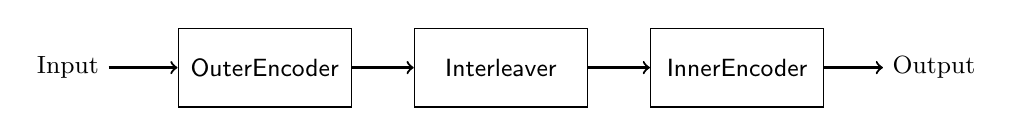
\begin{tikzpicture}[
  block/.style={rectangle, draw, minimum width=2.2cm, minimum height=1cm, font=\sffamily\small},
  node distance=2.5cm,
  font=\small
]
\node (input) {Input};
\node[block, right of=input, node distance=2.5cm] (outer) {Outer\\Encoder};
\node[block, right of=outer, node distance=3cm] (int) {Interleaver};
\node[block, right of=int, node distance=3cm] (inner) {Inner\\Encoder};
\node[right of=inner, node distance=2.5cm] (output) {Output};

\draw[->,thick] (input) -- (outer);
\draw[->,thick] (outer) -- (int);
\draw[->,thick] (int) -- (inner);
\draw[->,thick] (inner) -- (output);
\end{tikzpicture}
\end{center}

\textbf{Performance:}
\begin{itemize}
\item \textbf{Lower error floor} than PCCC (parallel turbo codes)
\item \textbf{Steeper waterfall} in BER curve
\item Better suited for very low BER requirements ($< 10^{-8}$)
\end{itemize}

\textbf{Decoding:} Iterative structure similar to PCCC, but information flows serially

\subsection{Repeat-Accumulate (RA) Codes}

\textbf{Structure:} Simplified turbo-like code with lower implementation complexity

\begin{center}
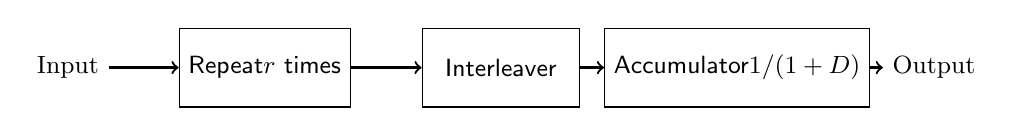
\begin{tikzpicture}[
  block/.style={rectangle, draw, minimum width=2cm, minimum height=1cm, font=\sffamily\small},
  node distance=2.5cm,
  font=\small
]
\node (input) {Input};
\node[block, right of=input, node distance=2.5cm] (repeat) {Repeat\\$r$ times};
\node[block, right of=repeat, node distance=3cm] (int) {Interleaver};
\node[block, right of=int, node distance=3cm] (accum) {Accumulator\\$1/(1+D)$};
\node[right of=accum, node distance=2.5cm] (output) {Output};

\draw[->,thick] (input) -- (repeat);
\draw[->,thick] (repeat) -- (int);
\draw[->,thick] (int) -- (accum);
\draw[->,thick] (accum) -- (output);
\end{tikzpicture}
\end{center}

\textbf{Accumulator:} Simplest possible RSC encoder with generator $G(D) = 1/(1+D)$

\textbf{Advantages:}
\begin{itemize}
\item Extremely simple encoder (just repetition + single-bit accumulator)
\item Near-turbo performance with much lower complexity
\item Easy hardware implementation
\end{itemize}

\textbf{Performance:} Within 1~dB of classical turbo codes, making them attractive for low-cost applications

\section{Applications}

Turbo codes have been deployed in numerous communication systems requiring near-capacity performance.

\subsection{3G UMTS (WCDMA)}

\textbf{Specification:} 3GPP TS 25.212

\textbf{Turbo code parameters:}
\begin{itemize}
\item Code rate: 1/3 (parent code)
\item Constraint length: $K = 4$ (16 states)
\item Generator polynomials: $G = [1, 13/15]_8$ (octal)
\item Interleaver: Length 40--5,114 bits (variable)
\item Iterations: 8 (typical)
\end{itemize}

\textbf{Channels:} Data channels (DPCH, HS-DSCH)

\textbf{Data rates:} 64~kbps to 2~Mbps (Release 99), up to 14.4~Mbps (HSPA)

\textbf{Performance:} BER $10^{-6}$ at $E_b/N_0 \approx 1.5$~dB (rate 1/3)

\subsection{4G LTE}

\textbf{Specification:} 3GPP TS 36.212

\textbf{Turbo code parameters:}
\begin{itemize}
\item Code rate: 1/3 (parent code)
\item Constraint length: $K = 4$
\item Generator polynomials: $G = [13, 15]_8$ (octal, systematic omitted)
\item Interleaver: QPP (Quadratic Permutation Polynomial) for contention-free parallel access
\item Iterations: 6--8 (adaptive, with early stopping)
\end{itemize}

\textbf{Data rates:}
\begin{itemize}
\item LTE Cat 3: Up to 100~Mbps downlink
\item LTE Cat 6: Up to 300~Mbps downlink
\item LTE-Advanced Cat 16: Up to 1~Gbps downlink
\end{itemize}

\textbf{Block sizes:} 40--6,144 bits (variable to match transport block size)

\textbf{Rate matching:} Adaptive puncturing (rates 1/2, 2/3, 3/4, 5/6) based on modulation and coding scheme (MCS)

\subsection{Deep Space Communications}

\textbf{NASA/ESA Standard:} CCSDS 131.0-B-3

\textbf{Mars Exploration Rovers (Spirit, Opportunity, Curiosity):}
\begin{itemize}
\item Turbo code rate: 1/6 (very robust for deep space)
\item Constraint length: $K = 5$ (32 states)
\item Interleaver: 65,536 bits (maximum capacity)
\item Iterations: 15 (no power constraints on ground receiver)
\end{itemize}

\textbf{Performance:} BER $< 10^{-8}$ at $E_b/N_0 \approx 0$~dB

\textbf{Data rate:} 128~kbps (from Mars surface, 225 million km away)

\textbf{Critical advantage:} Enables reliable communication with received power levels of $-200$~dBm or lower

\subsection{DVB-RCS (Satellite Return Channel)}

\textbf{Standard:} ETSI EN 301 790

\textbf{Turbo code:} Duo-binary turbo code
\begin{itemize}
\item Code rates: 1/3, 1/2, 2/3, 3/4, 4/5, 5/6, 6/7 (punctured)
\item Block sizes: 48--1,504 bits (variable)
\item Iterations: 6--8
\end{itemize}

\textbf{Application:} Interactive satellite broadband uplink (e.g., two-way Internet via satellite)

\textbf{Benefit:} Duo-binary structure provides lower error floor, critical for high-rate punctured codes

\subsection{Military Communications}

Turbo codes are widely used in military tactical data links:

\textbf{Link 16 (JTIDS):} Tactical data link for NATO forces
\begin{itemize}
\item Turbo coding for enhanced throughput modes
\item Supports low-probability-of-intercept (LPI) waveforms
\item Integrated with frequency hopping and DSSS
\end{itemize}

\textbf{MUOS (Mobile User Objective System):}
\begin{itemize}
\item Next-generation military satellite communications
\item Turbo codes for uplink and downlink
\item Supports mobile users with small antennas
\end{itemize}

\section{Implementation Complexity}

\subsection{Encoder Complexity}

Turbo encoding has \textbf{linear complexity} in the block length:

\begin{equation}
\mathcal{C}_{\text{enc}} = O(K \cdot N)
\end{equation}

where $K$ is the constraint length and $N$ is the block length.

\textbf{Example: $K=4$, rate 1/3, $N=1{,}000$ bits}
\begin{itemize}
\item 2 RSC encoders (16 states each)
\item Interleaver (memory read/write)
\item \textbf{Total:} $\sim$10--20 operations per bit
\item \textbf{Total operations:} $\sim$10,000--20,000 per block
\end{itemize}

\textbf{Hardware implementation:}
\begin{itemize}
\item Simple: Shift registers + XOR gates
\item Low gate count ($< 10{,}000$ gates for $K=4$)
\item High throughput possible (Gbps range)
\item Interleaver requires memory (RAM or lookup table)
\end{itemize}

\subsection{Decoder Complexity}

BCJR decoding dominates computational cost:

\begin{equation}
\mathcal{C}_{\text{dec}} = O(2^K \cdot N \cdot I)
\end{equation}

where $I$ is the number of iterations (typically 4--10).

\textbf{Example: $K=4$, 8 iterations, $N=1{,}000$ bits}
\begin{itemize}
\item 16 states per trellis stage
\item $\sim$50 operations per state per iteration
\item \textbf{Operations per bit per iteration:} $16 \times 50 = 800$
\item \textbf{Total operations per bit:} $800 \times 8 = 6{,}400$
\item \textbf{Total operations per block:} $\sim$6.4 million
\end{itemize}

\textbf{Decoder alternatives:}
\begin{itemize}
\item \textbf{BCJR (MAP):} Optimal performance, high complexity
\item \textbf{Log-MAP:} Near-optimal, numerically stable
\item \textbf{Max-Log-MAP:} $\sim$50\% complexity reduction, $\sim$0.3~dB loss
\item \textbf{SOVA:} $\sim$40\% of BCJR complexity, $\sim$0.3~dB loss
\end{itemize}

\subsection{Optimization Techniques}

\textbf{1. Max-Log-MAP Approximation}

Replace Jacobian logarithm with simpler max operation:
\begin{equation}
\log(e^a + e^b) \approx \max(a, b)
\end{equation}

\begin{itemize}
\item \textbf{Complexity reduction:} 50\%
\item \textbf{Performance loss:} $\sim$0.3~dB
\item \textbf{Benefit:} Eliminates lookup tables and transcendental functions
\end{itemize}

\textbf{2. Sliding Window Decoding}

Process trellis in fixed-size windows rather than entire block:
\begin{itemize}
\item \textbf{Memory reduction:} From $O(N)$ to $O(W)$ where $W$ is window size
\item \textbf{Throughput:} Enables pipelining
\item \textbf{Performance loss:} Negligible for $W > 5K$ (5 times constraint length)
\end{itemize}

\textbf{3. Early Termination (Stopping Criteria)}

Stop iterating when convergence detected, saving power and latency:

\textbf{Criteria:}
\begin{enumerate}
\item \textbf{LLR magnitude:} $|L(d_k)| > T$ for all $k$ (high confidence)
\item \textbf{Cross-entropy:} $H(L^{(i)}, L^{(i-1)}) < \epsilon$ (no significant change)
\item \textbf{CRC check:} If cyclic redundancy check passes, stop (used in LTE)
\end{enumerate}

\textbf{Benefit:} Average 3--5 iterations (vs. 8 worst-case) $\rightarrow$ 40\% power savings

\textbf{4. Radix-4 Processing}

Process 2 bits simultaneously:
\begin{itemize}
\item \textbf{Throughput:} $2\times$ speedup
\item \textbf{Trade-off:} $4\times$ states ($2^{2(K-1)}$), higher complexity per stage
\item \textbf{Use case:} High-throughput applications (e.g., LTE-Advanced)
\end{itemize}

\section{Error Floor Phenomenon}

\subsection{Causes}

The \textbf{error floor} is a region where BER stops improving (flattens) despite increasing SNR.

\textbf{Root cause:} Low-weight codewords with small free distance $d_{\text{free}}$

\textbf{Mechanism:} Specific input sequences produce low-weight outputs in \textbf{both} encoders:
\begin{itemize}
\item Input sequence with weight $w_{\text{in}} = 2$
\item Encoder 1 output weight: $w_1 = 4$
\item Encoder 2 output weight: $w_2 = 4$ (after interleaving)
\item Combined codeword weight: $d_{\text{free}} = w_1 + w_2 = 8$ (poor)
\end{itemize}

At high SNR, these low-weight codewords dominate error events, creating the floor.

\subsection{Mitigation Strategies}

\textbf{1. Optimized Interleaver Design}
\begin{itemize}
\item S-random interleaver (prevents short-distance mappings)
\item Dithered interleaver (adds controlled randomness)
\item Objective: Avoid input patterns that produce low weight in both encoders
\end{itemize}

\textbf{2. Longer Interleaver}
\begin{itemize}
\item Larger $N$ reduces probability of pathological patterns
\item Floor typically improves by 1--2 orders of magnitude per 10$\times$ length increase
\item Example: $N = 10{,}000$ achieves floor at $10^{-8}$ vs. $N = 1{,}000$ at $10^{-6}$
\end{itemize}

\textbf{3. Increased Constraint Length}
\begin{itemize}
\item Larger $K$ increases $d_{\text{free}}$ of component codes
\item Example: $K = 5$ vs. $K = 4$ lowers floor by $\sim$1 order of magnitude
\item Trade-off: Decoder complexity grows as $O(2^K)$
\end{itemize}

\textbf{4. Post-Processing}
\begin{itemize}
\item Outer code (e.g., CRC) detects residual errors
\item ARQ (automatic repeat request) requests retransmission
\item Concatenation with Reed-Solomon outer code
\end{itemize}

\textbf{Typical error floors:}
\begin{itemize}
\item Standard turbo codes: $10^{-6}$ to $10^{-8}$
\item Optimized interleavers: $10^{-8}$ to $10^{-10}$
\item Duo-binary turbo codes: $10^{-10}$ to $10^{-12}$
\end{itemize}

\section{Comparison with Other Codes}

\subsection{Performance Comparison}

\begin{center}
\begin{tabular}{@{}lcccc@{}}
\toprule
Code & $E_b/N_0$ @ BER $10^{-5}$ & Gap to Shannon & Complexity & Latency \\
 & (rate 1/2) & Limit & & \\
\midrule
Uncoded BPSK & 9.6~dB & +11~dB & --- & Zero \\
Convolutional ($K=7$) & 4.5~dB & +6~dB & Low & Low \\
\textbf{Turbo} & \textbf{0.7~dB} & \textbf{+0.5~dB} & Moderate & Moderate \\
LDPC & 0.5~dB & +0.3~dB & Moderate & Low \\
Polar & 1.0~dB & +0.8~dB & Low & Low \\
\bottomrule
\end{tabular}
\end{center}

\textbf{Shannon limit for rate 1/2 BPSK:} $E_b/N_0 = -1.6$~dB (theoretical capacity limit)

\textbf{Turbo code advantages:}
\begin{itemize}
\item Near-Shannon limit performance (within 0.5~dB)
\item Proven technology with extensive deployment
\item Standardized in 3G/4G cellular systems
\item Flexible rate adaptation through puncturing
\end{itemize}

\textbf{Turbo code disadvantages:}
\begin{itemize}
\item Higher latency due to iterative decoding
\item Error floor phenomenon at high SNR
\item Serial trellis processing limits parallelism
\item Being replaced by LDPC in newer standards (5G, WiFi 6)
\end{itemize}

\subsection{Turbo vs. LDPC Codes}

Direct comparison with the modern alternative:

\begin{center}
\begin{tabular}{@{}lll@{}}
\toprule
Aspect & Turbo Codes & LDPC Codes \\
\midrule
$E_b/N_0$ @ BER $10^{-5}$ & 0.7~dB & 0.5~dB \\
Error floor & $10^{-7}$ typical & $10^{-12}$ possible \\
Decoding latency & High (serial iterations) & Lower (parallel belief prop.) \\
Complexity & Moderate ($\sim$6,000 ops/bit) & Moderate ($\sim$5,000 ops/bit) \\
Hardware architecture & Serial (trellis) & Parallel (bipartite graph) \\
Standardization & 3G UMTS, 4G LTE & 5G NR, WiFi 6, DVB-S2 \\
Rate flexibility & Puncturing patterns & Structured parity matrices \\
Implementation maturity & Very mature (20+ years) & Mature (10+ years) \\
\bottomrule
\end{tabular}
\end{center}

\textbf{Industry trend:} LDPC codes are replacing turbo codes in new standards due to:
\begin{itemize}
\item Lower error floor (critical for high data rates)
\item Better parallelization (higher throughput)
\item Lower latency (fewer iterations, inherent parallelism)
\item More flexible structure (QC-LDPC allows various rates)
\end{itemize}

However, turbo codes remain widely deployed in existing 3G/4G infrastructure and will continue operating for decades.

\section{Design Guidelines}

\subsection{When to Choose Turbo Codes}

Turbo codes are optimal for:

\begin{enumerate}
\item \textbf{Near-capacity performance critical}
  \begin{itemize}
  \item Applications requiring $< 1$~dB from Shannon limit
  \item Power-limited systems (satellite, deep space)
  \item High-reliability requirements at low SNR
  \end{itemize}

\item \textbf{Moderate block sizes}
  \begin{itemize}
  \item Typical range: 1,000--10,000 bits
  \item Sweet spot for interleaver effectiveness
  \item Not suitable for very short packets ($< 100$ bits)
  \end{itemize}

\item \textbf{Latency acceptable}
  \begin{itemize}
  \item Iterative decoding introduces delay (4--10 iterations)
  \item Not critical-path for user experience
  \item Throughput more important than latency
  \end{itemize}

\item \textbf{Error floor $10^{-6}$--$10^{-8}$ sufficient}
  \begin{itemize}
  \item Acceptable for voice, video, data
  \item CRC + ARQ can handle residual errors
  \item Not suitable for ultra-reliable low-latency (URLLC)
  \end{itemize}

\item \textbf{Existing infrastructure}
  \begin{itemize}
  \item Leverage 3G/4G standardization
  \item Mature implementations available
  \item Interoperability with existing systems
  \end{itemize}
\end{enumerate}

\subsection{When to Avoid Turbo Codes}

Consider alternatives if:

\begin{enumerate}
\item \textbf{Ultra-low error floor needed} ($< 10^{-10}$) $\rightarrow$ Use LDPC or duo-binary turbo

\item \textbf{Low latency critical} (e.g., URLLC in 5G) $\rightarrow$ Use LDPC or polar codes

\item \textbf{Very short blocks} ($< 100$ bits) $\rightarrow$ Use polar codes or convolutional codes

\item \textbf{New system design} (future-proof) $\rightarrow$ Consider LDPC (5G/WiFi 6 standard)

\item \textbf{High parallelism required} $\rightarrow$ LDPC offers better parallel processing
\end{enumerate}

\section{Summary}

\begin{center}
\begin{tabular}{@{}ll@{}}
\toprule
\textbf{Parameter} & \textbf{Value/Description} \\
\midrule
Discovery & 1993 (Berrou, Glavieux, Thitimajshima) \\
Key innovation & Parallel concatenation + iterative decoding \\
Code rate & 1/3 (parent), flexible via puncturing \\
Performance & $E_b/N_0 = 0.7$~dB @ BER $10^{-5}$ (rate 1/2) \\
Gap to Shannon & 0.5~dB (unprecedented in 1993) \\
Encoder & Two RSC encoders + interleaver \\
Decoder & BCJR (MAP) or SOVA (sub-optimal) \\
Iterations & Typically 4--10 \\
Complexity & Moderate (6,000 ops/bit, $K=4$, 8 iter.) \\
Latency & Moderate (iterative decoding) \\
Error floor & $10^{-6}$ to $10^{-8}$ typical \\
Block size & 1,000--10,000 bits (typical) \\
Applications & 3G, 4G LTE, deep space, satellite \\
\bottomrule
\end{tabular}
\end{center}

\textbf{Key takeaway:} Turbo codes revolutionized communication systems by achieving performance within 0.5~dB of the Shannon limit through iterative exchange of extrinsic information between two decoders. While being replaced by LDPC in 5G and WiFi 6 due to better error floors and parallelism, turbo codes remain the foundation of 3G/4G cellular systems serving billions of users worldwide.

\section{Python Implementation Example}

\begin{Shaded}
\begin{Highlighting}[]
\ImportTok{import}\NormalTok{ numpy }\ImportTok{as}\NormalTok{ np}

\KeywordTok{def}\NormalTok{ rsc\_encode(data, g\_fb}\OperatorTok{=}\NormalTok{[}\DecValTok{1}\NormalTok{,}\DecValTok{1}\NormalTok{,}\DecValTok{1}\NormalTok{], g\_ff}\OperatorTok{=}\NormalTok{[}\DecValTok{1}\NormalTok{,}\DecValTok{0}\NormalTok{,}\DecValTok{1}\NormalTok{]):}
    \CommentTok{"""RSC encoder (K=3 example)."""}
\NormalTok{    K }\OperatorTok{=} \BuiltInTok{len}\NormalTok{(g\_fb)}
\NormalTok{    state }\OperatorTok{=} \DecValTok{0}
\NormalTok{    systematic }\OperatorTok{=}\NormalTok{ []}
\NormalTok{    parity }\OperatorTok{=}\NormalTok{ []}
    
    \ControlFlowTok{for}\NormalTok{ bit }\KeywordTok{in}\NormalTok{ data:}
        \CommentTok{\# Feedback XOR}
\NormalTok{        fb }\OperatorTok{=}\NormalTok{ bit}
        \ControlFlowTok{for}\NormalTok{ i }\KeywordTok{in} \BuiltInTok{range}\NormalTok{(}\DecValTok{1}\NormalTok{, K):}
            \ControlFlowTok{if}\NormalTok{ g\_fb[i] }\KeywordTok{and}\NormalTok{ (state }\OperatorTok{\&}\NormalTok{ (}\DecValTok{1} \OperatorTok{\textless{}\textless{}}\NormalTok{ (i}\OperatorTok{{-}}\DecValTok{1}\NormalTok{))):}
\NormalTok{                fb }\OperatorTok{\^{}=} \DecValTok{1}
        
        \CommentTok{\# Parity XOR}
\NormalTok{        p }\OperatorTok{=} \DecValTok{0}
        \ControlFlowTok{for}\NormalTok{ i }\KeywordTok{in} \BuiltInTok{range}\NormalTok{(K):}
            \ControlFlowTok{if}\NormalTok{ i }\OperatorTok{==} \DecValTok{0}\NormalTok{:}
                \ControlFlowTok{if}\NormalTok{ g\_ff[}\DecValTok{0}\NormalTok{]:}
\NormalTok{                    p }\OperatorTok{\^{}=}\NormalTok{ fb}
            \ControlFlowTok{else}\NormalTok{:}
                \ControlFlowTok{if}\NormalTok{ g\_ff[i] }\KeywordTok{and}\NormalTok{ (state }\OperatorTok{\&}\NormalTok{ (}\DecValTok{1} \OperatorTok{\textless{}\textless{}}\NormalTok{ (i}\OperatorTok{{-}}\DecValTok{1}\NormalTok{))):}
\NormalTok{                    p }\OperatorTok{\^{}=} \DecValTok{1}
        
        \CommentTok{\# Update state (shift in feedback bit)}
\NormalTok{        state }\OperatorTok{=}\NormalTok{ ((state }\OperatorTok{\textless{}\textless{}} \DecValTok{1}\NormalTok{) }\OperatorTok{|}\NormalTok{ fb) }\OperatorTok{\&}\NormalTok{ ((}\DecValTok{1} \OperatorTok{\textless{}\textless{}}\NormalTok{ (K}\OperatorTok{{-}}\DecValTok{1}\NormalTok{)) }\OperatorTok{{-}} \DecValTok{1}\NormalTok{)}
        
\NormalTok{        systematic.append(bit)}
\NormalTok{        parity.append(p)}
    
    \ControlFlowTok{return}\NormalTok{ systematic, parity}

\KeywordTok{def}\NormalTok{ turbo\_encode(data, interleaver\_indices):}
    \CommentTok{"""Turbo encoder (rate 1/3)."""}
    \CommentTok{\# Encoder 1}
\NormalTok{    sys1, par1 }\OperatorTok{=}\NormalTok{ rsc\_encode(data)}
    
    \CommentTok{\# Interleave}
\NormalTok{    data\_int }\OperatorTok{=}\NormalTok{ [data[i] }\ControlFlowTok{for}\NormalTok{ i }\KeywordTok{in}\NormalTok{ interleaver\_indices]}
    
    \CommentTok{\# Encoder 2}
\NormalTok{    sys2, par2 }\OperatorTok{=}\NormalTok{ rsc\_encode(data\_int)}
    
    \CommentTok{\# Output: systematic + parity1 + parity2}
    \CommentTok{\# (sys1 and sys2 are same as data, use sys1)}
    \ControlFlowTok{return}\NormalTok{ sys1, par1, par2}

\CommentTok{\# Example}
\NormalTok{data }\OperatorTok{=}\NormalTok{ [}\DecValTok{1}\NormalTok{, }\DecValTok{0}\NormalTok{, }\DecValTok{1}\NormalTok{, }\DecValTok{1}\NormalTok{, }\DecValTok{0}\NormalTok{, }\DecValTok{1}\NormalTok{, }\DecValTok{0}\NormalTok{, }\DecValTok{0}\NormalTok{]}
\NormalTok{interleaver }\OperatorTok{=}\NormalTok{ [}\DecValTok{0}\NormalTok{, }\DecValTok{4}\NormalTok{, }\DecValTok{2}\NormalTok{, }\DecValTok{6}\NormalTok{, }\DecValTok{1}\NormalTok{, }\DecValTok{5}\NormalTok{, }\DecValTok{3}\NormalTok{, }\DecValTok{7}\NormalTok{]  }\CommentTok{\# S{-}random example}

\NormalTok{sys, par1, par2 }\OperatorTok{=}\NormalTok{ turbo\_encode(data, interleaver)}

\BuiltInTok{print}\NormalTok{(}\SpecialStringTok{f"Data:       }\SpecialCharTok{\{}\NormalTok{data}\SpecialCharTok{\}}\SpecialStringTok{"}\NormalTok{)}
\BuiltInTok{print}\NormalTok{(}\SpecialStringTok{f"Systematic: }\SpecialCharTok{\{}\NormalTok{sys}\SpecialCharTok{\}}\SpecialStringTok{"}\NormalTok{)}
\BuiltInTok{print}\NormalTok{(}\SpecialStringTok{f"Parity 1:   }\SpecialCharTok{\{}\NormalTok{par1}\SpecialCharTok{\}}\SpecialStringTok{"}\NormalTok{)}
\BuiltInTok{print}\NormalTok{(}\SpecialStringTok{f"Parity 2:   }\SpecialCharTok{\{}\NormalTok{par2}\SpecialCharTok{\}}\SpecialStringTok{"}\NormalTok{)}
\BuiltInTok{print}\NormalTok{(}\SpecialStringTok{f"Code rate:  }\SpecialCharTok{\{}\BuiltInTok{len}\NormalTok{(data)}\SpecialCharTok{\}}\SpecialStringTok{/}\SpecialCharTok{\{}\BuiltInTok{len}\NormalTok{(sys)}\OperatorTok{+}\BuiltInTok{len}\NormalTok{(par1)}\OperatorTok{+}\BuiltInTok{len}\NormalTok{(par2)}\SpecialCharTok{\}}\SpecialStringTok{ = 1/3"}\NormalTok{)}
\end{Highlighting}
\end{Shaded}

\textbf{Note:} Full iterative decoder (BCJR) is complex ($\sim$200+ lines). Use production libraries like \texttt{commpy}, \texttt{sionna}, or vendor-specific implementations for real applications.

\section{Further Reading}

This chapter connects to several related topics in the book:

\textbf{Foundational concepts:}
\begin{itemize}
\item \textbf{Chapter 4: Convolutional Codes \& Viterbi Decoding}---RSC encoders are the building blocks of turbo codes
\item \textbf{Chapter 6: Forward Error Correction (FEC)}---General overview of error correction techniques
\item \textbf{Chapter 8: Bit Error Rate (BER)}---Performance metrics and analysis methods
\item \textbf{Chapter 2: Shannon's Channel Capacity Theorem}---Theoretical limits that turbo codes approach
\end{itemize}

\textbf{Advanced error correction:}
\begin{itemize}
\item \textbf{Chapter 5: LDPC Codes}---Modern alternative with lower error floor (5G, WiFi 6)
\item \textbf{Chapter 7: Polar Codes}---Provably capacity-achieving codes (5G control channels)
\item \textbf{Chapter 3: Block Codes (Hamming, BCH, Reed-Solomon)}---Simpler algebraic codes
\end{itemize}

\textbf{Modulation and system design:}
\begin{itemize}
\item \textbf{Chapter 12: QPSK Modulation}---Common modulation used with turbo codes
\item \textbf{Chapter 18: Adaptive Modulation \& Coding (AMC)}---Dynamic code rate selection
\item \textbf{Chapter 22: Complete Link Budget Analysis}---System-level design including coding gain
\end{itemize}

\textbf{Applications:}
\begin{itemize}
\item \textbf{Chapter 25: Real-World System Examples}---Practical turbo code deployments
\item \textbf{Chapter 16: Signal Chain (End-to-End Processing)}---Integration of turbo coding in communication systems
\end{itemize}
